\documentclass[tikz,border=1mm]{standalone}
\usepackage[T1]{fontenc}
\usepackage{lmodern}
\usepackage{amsmath,amssymb}
\usetikzlibrary{arrows.meta}
\pdfvariable suppressoptionalinfo 767\relax

\definecolor{navy}{HTML}{17486D}
\definecolor{teal}{HTML}{145B54}
\definecolor{rust}{HTML}{A14029}
\definecolor{slate}{HTML}{354758}
\definecolor{rulegray}{HTML}{CAD5DC}
\newcommand{\sort}{\operatorname{sort}}
\newcommand{\key}{\operatorname{key}}

\begin{document}
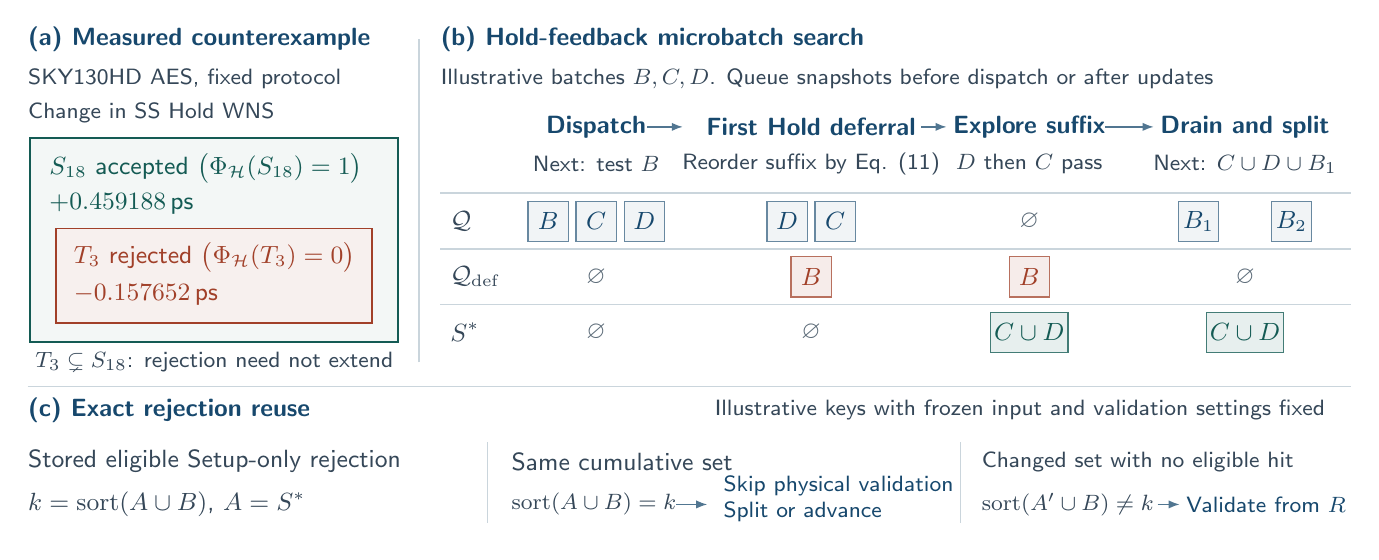
\begin{tikzpicture}[x=1mm, y=1mm, font=\sffamily\small, text=slate,
  heading/.style={anchor=west,font=\sffamily\bfseries\small,inner sep=0pt,text=navy},
  start/.style={anchor=west,inner sep=0pt},
  stage/.style={font=\sffamily\bfseries\small,inner sep=0pt,text=navy},
  detail/.style={font=\sffamily\footnotesize,inner sep=0pt},
  tile/.style={draw=navy!65,fill=navy!6,text=navy,minimum size=5.1mm,
    line width=.45pt,inner sep=.45mm,font=\sffamily\small},
  deferred/.style={tile,draw=rust!75,fill=rust!10,text=rust},
  accepted/.style={tile,draw=teal!80,fill=teal!10,text=teal},
  empty/.style={text=slate!80,inner sep=0pt},
  edge/.style={-{Latex[length=1.4mm]},line width=.5pt,draw=navy!75},
  separator/.style={line width=.45pt,draw=rulegray}]
\path[use as bounding box] (0,0) rectangle (168,64);

% Panel (a). WINDOW_RULE_SCOPE.md uses the frozen physical receipts.
% Baseline SS Hold WNS: 55.29576796448055 ps. T3: 55.138116294983774 ps.
% S18: 55.75495620746551 ps. See Stage 1 JSON, part1_counterexample_and_timing_audit.
\node[heading] at (0,62.5) {(a) Measured counterexample};
\node[start,detail] at (0,57.5) {SKY130HD AES, fixed protocol};
\node[start,detail] at (0,53.2) {Change in SS Hold WNS};

\draw[teal,line width=.7pt,fill=teal!5] (0.35,24.1) rectangle (47,50);
\node[start,text=teal] at (2.7,46.15) {\(S_{18}\) accepted \(\bigl(\Phi_{\mathcal H}(S_{18})=1\bigr)\)};
\node[start,text=teal] at (2.7,41.65) {\(+0.459188\)\,ps};
\draw[rust,line width=.65pt,fill=rust!8] (3.6,26.5) rectangle (43.7,38.5);
\node[start,text=rust] at (5.8,34.8) {\(T_3\) rejected \(\bigl(\Phi_{\mathcal H}(T_3)=0\bigr)\)};
\node[start,text=rust] at (5.8,30.1) {\(-0.157652\)\,ps};
\node[detail] at (23.7,21.5) {\(T_3\subsetneq S_{18}\): rejection need not extend};

% Panel (b). Symbolic states only. B, C and D are multi-gate batches.
% Show both halves entering Q before dispatch; outcome of the renewed check is open.
\draw[separator] (49.7,21.5) -- (49.7,62.5);
\node[heading] at (52.4,62.5) {(b) Hold-feedback microbatch search};
\node[start,detail] at (52.4,57.5) {Illustrative batches \(B,C,D\). Queue snapshots before dispatch or after updates};

\node[stage] at (72.2,51.4) {Dispatch};
\node[stage] at (99.5,51.4) {First Hold deferral};
\node[stage] at (127.2,51.4) {Explore suffix};
\node[stage] at (154.6,51.4) {Drain and split};
\draw[edge] (78.7,51.4) -- (83.2,51.4);
\draw[edge] (113.5,51.4) -- (116.7,51.4);
\draw[edge] (136.8,51.4) -- (143.0,51.4);

\node[detail] at (72.2,46.7) {Next: test \(B\)};
\node[detail] at (99.5,46.7) {Reorder suffix by Eq. (11)};
\node[detail] at (127.2,46.7) {\(D\) then \(C\) pass};
\node[detail] at (154.6,46.7) {Next: \(C\cup D\cup B_1\)};

\draw[separator] (52.4,43.0) -- (168,43.0);
\draw[separator] (52.4,35.9) -- (168,35.9);
\draw[separator] (52.4,28.8) -- (168,28.8);

\node[start] at (53.6,39.4) {\(\mathcal Q\)};
\node[start] at (53.6,32.35) {\(\mathcal Q_{\mathrm{def}}\)};
\node[start] at (53.6,25.3) {\(S^*\)};

\node[tile] at (66.1,39.4) {\(B\)};
\node[tile] at (72.2,39.4) {\(C\)};
\node[tile] at (78.3,39.4) {\(D\)};
\node[tile] at (96.45,39.4) {\(D\)};
\node[tile] at (102.55,39.4) {\(C\)};
\node[empty] at (127.2,39.4) {\(\varnothing\)};
\node[tile] at (148.7,39.4) {\(B_1\)};
\node[tile] at (160.5,39.4) {\(B_2\)};

\node[empty] at (72.2,32.35) {\(\varnothing\)};
\node[deferred] at (99.5,32.35) {\(B\)};
\node[deferred] at (127.2,32.35) {\(B\)};
\node[empty] at (154.6,32.35) {\(\varnothing\)};

\node[empty] at (72.2,25.3) {\(\varnothing\)};
\node[empty] at (99.5,25.3) {\(\varnothing\)};
\node[accepted] at (127.2,25.3) {\(C\cup D\)};
\node[accepted] at (154.6,25.3) {\(C\cup D\)};

% Panel (c). The normal microbatch example uses eligible Setup-only rejections.
% A changed key is checked when it has no eligible cache entry of its own.
\draw[separator] (0,18.45) -- (168,18.45);
\node[heading] at (0,15.4) {(c) Exact rejection reuse};
\node[start,detail] at (87.2,15.4) {Illustrative keys with frozen input and validation settings fixed};

\draw[separator] (58.4,1.1) -- (58.4,11.4);
\draw[separator] (118.5,1.1) -- (118.5,11.4);
\node[start] at (0,8.9) {Stored eligible Setup-only rejection};
\node[start] at (0,3.45) {\(k=\sort(A\cup B)\), \(A=S^*\)};
\node[start] at (61.4,8.9) {Same cumulative set};
\node[start,detail] at (61.4,3.45) {\(\sort(A\cup B)=k\)};
\draw[edge] (82.4,3.45) -- (86.3,3.45);
\node[start,detail,text=navy] at (88.3,5.85) {Skip physical validation};
\node[start,detail,text=navy] at (88.3,2.55) {Split or advance};
\node[start,detail] at (121.1,8.9) {Changed set with no eligible hit};
\node[start,detail] at (121.1,3.45) {\(\sort(A'\cup B)\ne k\)};
\draw[edge] (143.5,3.45) -- (146.3,3.45);
\node[start,detail,text=navy] at (147.1,3.45) {Validate from \(R\)};
\end{tikzpicture}
\end{document}\n